\chapter{Разработка и формализация нового алгоритма построения выпуклой оболочки} \label{chapt2}

\section{Формализация понятия выпуклой оболочки} \label{sect2_1}

\section{Описание алгоритма основанного на использовании бинарного дерева} \label{sect2_2}

\subsection{Основная идея} \label{subsect2_2_1}

Основная идея предлагаемого алгоритма очень похожа на принцип, лежащий в основе инкрементального алгоритма. Мы можем хранить точки в сбалансированном по высоте двоичном дереве поиска. Главное различие с инкрементальным алгоритмом - точки будут храниться в одном дереве, где точки будут расположены по углу относительно центра выпуклой оболочки.

Чтобы объяснить работу алгоритма нам понадобится уже известный нам предикат $ccw$, определённый в формуле \ref{eq:ccw}. Также необходимо определить понятие экстремальной точки. Экстремальная точка множества $S$ - это точка, которая точно принадлежит выпуклой оболочке $S$.

Пусть дано множество точек $S$ и необходимо найти выпуклую оболочку данного множества.

Первый шаг алгоритма - это нахождение приближенного центра, с помощью которого будут отсортированы в дереве точки. Это можно сделать посчитав среднее арифметическое трёх экстремальных точек. Это отличная аппроксимация центра для наших целей. Первые 2 экстремальные точки -  это самая левая $A$ и правая $B$ точки множества $S$. Третья точка - это наиболее удалённая от линии $A, B$ точка $C$.

Пример таких точек показан на рисунке \ref{img:my_extreme_points}. Точка $D$ - это приближённый центр выпуклой оболочки, который мы искали.

\begin{figure}[H]
	{\centering
		\hfill
		\subbottom[\label{img:my_extreme_points_1}]{%
			\includegraphics[width=0.4\linewidth]{my_extreme_points_1}}
		\hfill
		\subbottom[\label{img:my_extreme_points_2}]{%
			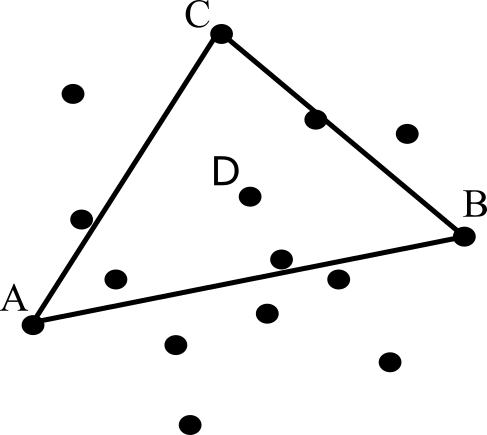
\includegraphics[width=0.4\linewidth]{my_extreme_points_2}}
		\hfill
	}
	\caption{Нахождение приближённого центра выпуклой оболочки}
	\label{img:my_extreme_points}
\end{figure}

После нахождения центра мы добавляем точки $A, B, C$ в наше дерево поиска. Остальные точки будут добавлены в случайном порядке.

Пусть мы уже построили дерево поиска, в котором содержится наша выпуклая оболочка, отсортированная по углу относительно центра $D$, найденного ранее. Теперь необходимо добавить новую точку $A$.

Первое, что необходимо найти - это две точки $L$ и $R$. Точки $L$, $R$ - это точки слева и справа соответственно от $A$ по углу относительно центра $D$.

%TODO: Проверить, что я точно написал правду для точек на одной прямой

После чего может быть 2 случая. Если $ccw(L, R, A)$ не выполняется, то новая точка $A$ не должна быть частью выпуклой оболочки и может быть пропущена. Этот случай показан на рисунке \ref{img:my_point_cases_1}. Иначе точки должна быть частью выпуклой оболочки и мы продолжим добавлять её. Это показано на рисунке \ref{img:my_point_cases_2}.

\begin{figure}[H]
	{\centering
		\hfill
		\subbottom[\label{img:my_point_cases_1}]{%
			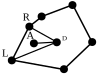
\includegraphics[width=0.4\linewidth]{my_add_point_1}}
		\hfill
		\subbottom[\label{img:my_point_cases_2}]{%
			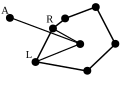
\includegraphics[width=0.4\linewidth]{my_add_point_2}}
		\hfill
	}
	\caption{Добавление новой точки в выпуклую оболочку}
	\label{img:my_point_cases}
\end{figure}

Итак, мы определили, что точка $A$ должна быть на выпуклой оболочке. Теперь необходимо удалить точки, которые будут внутри оболочки после добавления точки $A$. Это делается с помощью итерации по точкам вправо (аналогичный алгоритм должен быть выполнен для левой стороны) от новой точки. Чтобы определить должна ли точка быть удалена или нет мы будем использовать подход, похожий на тот, который используется в алгоритме Грэхема. Каждые два смежных ребра выпуклой оболочки должны лежать против часовой стрелки.

Пусть следующая точка, которая рассматривается на удаление - это $B$, а точка следующая после неё $C$. Как сказано выше каждые два смежных ребра должны лежать против часовой стрелки. Это очень легко проверить с помощью предиката $ccw$. Если $ccw(C, B, A)$ тогда $B$ не должна быть удалена и мы должны прекратить удаление точек в эту сторону, потому что все точки после $B$ уже удовлетворяют условию выпуклой оболочки. Иначе мы должны удалить точку $B$ и рассмотреть точку $C$ как следующую. Этот процесс показан на рисунках \ref{img:my_points_deletion_1} и \ref{img:my_points_deletion_2}.

На рисунках \ref{img:my_points_deletion_1_1} и \ref{img:my_points_deletion_1_2} можно видеть, что точки $C, B, A$ лежат по часовой стрелке, поэтому точка $B$ должна быть удалена из выпуклой оболочки. Рисунок \ref{img:my_points_deletion_2_1} демонстрирует, что мы должна прекратить удаление точек справа от новой точки, так как $C, B, A$ теперь формирует тройку, которая лежит против часовой стрелки. Аналогично удаление не нужно производить слева от точки, что показано на рисунке \ref{img:my_points_deletion_2_2}. Действительно, на рисунках видно, что в конце получилась готовая выпуклая оболочка добавленных на текущий момент точек.

\begin{figure}[H]
	{\centering
		\hfill
		\subbottom[\label{img:my_points_deletion_1_1}]{%
			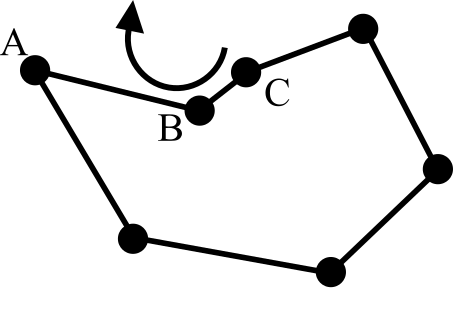
\includegraphics[width=0.4\linewidth]{my_add_point_3}}
		\hfill
		\subbottom[\label{img:my_points_deletion_1_2}]{%
			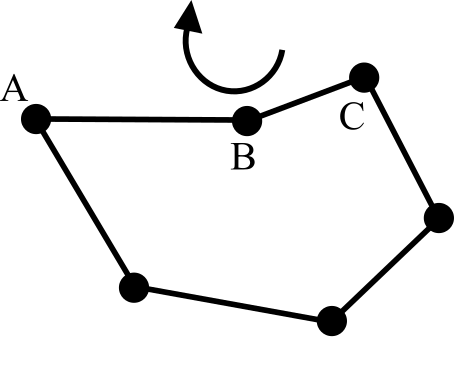
\includegraphics[width=0.4\linewidth]{my_add_point_4}}
		\hfill
	}
	\caption{Удаление точек, которые оказались внутри выпуклой оболочки}
	\label{img:my_points_deletion_1}
\end{figure}

\begin{figure}[H]
	{\centering
		\hfill
		\subbottom[\label{img:my_points_deletion_2_1}]{%
			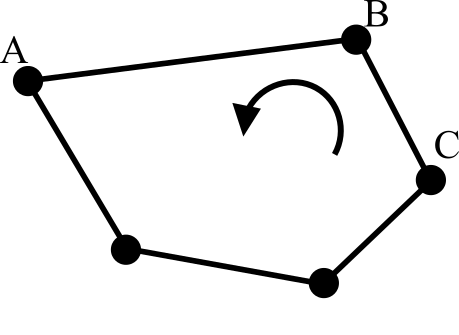
\includegraphics[width=0.4\linewidth]{my_add_point_5}}
		\hfill
		\subbottom[\label{img:my_points_deletion_2_2}]{%
			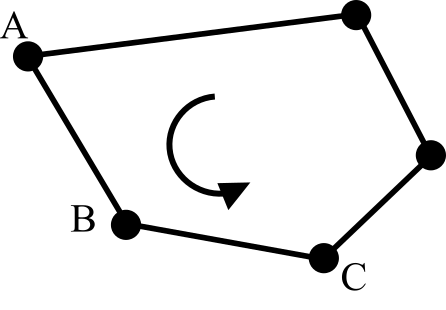
\includegraphics[width=0.4\linewidth]{my_add_point_6}}
		\hfill
	}
	\caption{Критерий завершения удаления точек}
	\label{img:my_points_deletion_2}
\end{figure}

Как видно этот процесс очень схож с процессом добавления точек в инкрементальном алгоритме. Различия небольшие, но они позволяют быстрее добавлять точки в выпуклую оболочку.

Блок-схема всего алгоритма показана на рисунках \ref{img:my_algo} и \ref{img:my_algo_deletion}.

\begin{figure}[H]
	\centering
	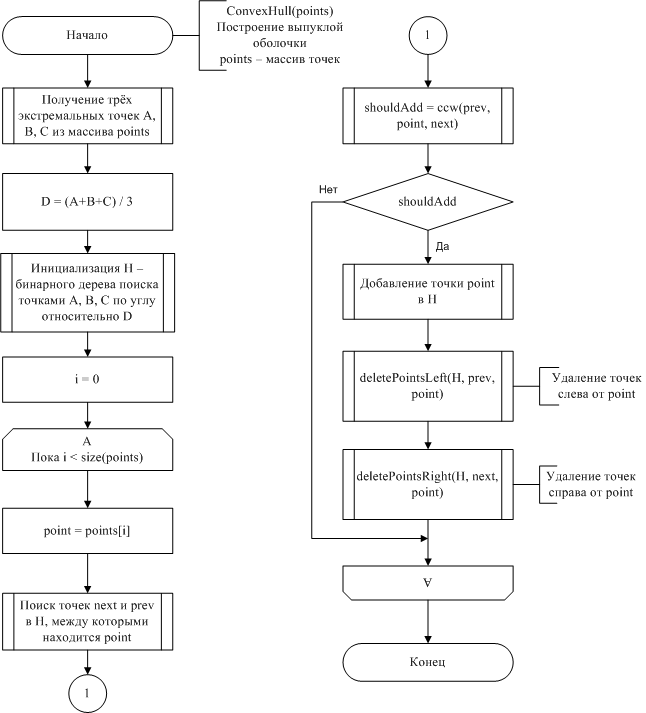
\includegraphics[scale=0.8]{my_algo}
	\caption{Блок-схема работы предлагаемого алгоритма}
	\label{img:my_algo}
\end{figure}

\begin{figure}[H]
	\centering
	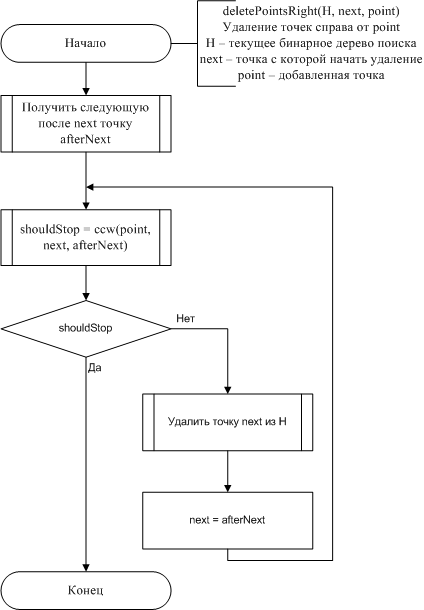
\includegraphics[scale=0.8]{my_algo_2}
	\caption{Блок-схема функции удаления точек перед добавлением точки point}
	\label{img:my_algo_deletion}
\end{figure}

\subsection{Детали реализации} \label{subsect2_2_2}

Первая важная деталь, которая упрощает реализацию нашего алгоритма - это конечно преобразование точек при работе алгоритма. Намного удобнее работать считать, что приближённый центр $D$, получение которого описывалось в предыдущей главе - это точка $0, 0)$. Как показано в \ref{eq:ccw} мы вычисляем $ccw$ через $det$, а вычислять $det(A, B, D)$ легче, если $D_x = 0$ и $D_y = 0$. Также нельзя забывать про конечную цель вычисления выпуклой оболочки. Для вычисления дескриптора опять намного удобнее пользоваться координатами уже переведёнными в центр объекта, так как на дескриптор никак не должно влиять положения объекта на изображении.

Вторая деталь, которая также важна при реализации - это углы относительно центра, про которые мы так много говорили. Вычисление углов через тригонометрические операции - это очень долго, и в этом случае наш алгоритм не смог бы конкурировать по производительности с самыми популярными алгоритмами вычисления выпуклой оболочки.

Необходимо придумать предикат, который бы определял положение точек в дереве, которое хранит текущую выпуклую оболочку. Первой попыткой придумать такой предикат будет использование предиката $ccw$, как это показано в \ref{eq:my_ccw_predicate}.

\begin{equation}\label{eq:my_ccw_predicate}
A<B=ccw(A, B, (0, 0))
\end{equation}

Заметим, что можно использовать точку $(0, 0)$ как центр, так как точки $A, B$ уже преобразованы в новую систему координат.

%TODO: перевести strict weak ordering и добавить ссылку на стандарт c++
К сожалению, такой предикат не соответствует strict weak ordering, потому что не выполняется транзитивность. Как можно видеть на рисунке ... 

%TODO: add pitcure here

Итак, необходимо сделать такую функцию, которая принимает точки $A$ и $B$ и возвращает $true$, если $A$ меньше $B$, иначе возвращает $false$. Эта функция будет использована в сбалансированном дереве поиска как компаратор. Был использован следующий алгоритм:

\begin{algorithm}[H]
	\caption{BSTPredicate - компаратор, используемый для сравнения точек}
	\label{alg:bst_predicate}
	\begin{algorithmic}[1]
		\Procedure{BSTPredicate}{$A, B$}
		\State $leftUp \gets 0<y_A$
		\State $rightUp \gets 0<y_B$
		\If {$leftUp \neq rightUp$}
			\Return $leftUp < rightUp$
		\EndIf
		\If {$(y_A=0) \& (y_B=0)$}
			\Return $(0<x_A) < (0<x_B)$
		\EndIf
		\Return $ccw(A, B, (0, 0))$
		\EndProcedure
	\end{algorithmic}
\end{algorithm}

\section{Доказательство корректности работы алгоритма} \label{subsect2_3}

\section{Оценка быстродействия предлагаемого алгоритма} \label{subsect2_4}


